\documentclass[10pt,compress,t,notes=noshow,xcolor=table]{beamer}

\input{../../style/preamble}
\input{../../latex-math/basic-math}
\input{../../latex-math/basic-ml}

\title{Interpretable Machine Learning}

\begin{document}

\titlemeta{
Feature Effects
}{
ALE: Conclusions, Limitations, and Follow-up Work
}{
figure/ale_plot.pdf
}{
\item Summarize what ALE achieves and where its approximation can struggle
\item Understand the intuition behind DALE and RHALE
\item Choose an appropriate method and find the follow-up literature
}


\begin{framev}[align=top]{ALE: Main Conclusion \furtherreading{APLEYZHU2020}}
ALE provides a useful global summary of how a feature affects model predictions in data-supported regions.
\spacer[0.25]
\begin{itemizeM}
\item It averages \textbf{local changes} in predictions rather than predictions themselves.
\item It respects feature dependencies by averaging locally over observed data.
\item It avoids much of the extrapolation problem of PD plots and the omitted-variable problem of marginal plots.
\item Its centered curve answers: \textit{Where does this feature increase or decrease the prediction relative to its average effect?}
\end{itemizeM}
\spacer[0.25]
\textbf{Important distinction:} The ALE definition is conceptually attractive, but its finite-sample approximation and its global averaging still have limitations.
\end{framev}


\begin{framev}[align=top]{What Is Left to Improve?}
\begin{center}
\renewcommand{\arraystretch}{1.35}
\begin{tabular}{p{0.25\textwidth} p{0.42\textwidth} p{0.19\textwidth}}
\toprule
\textbf{ALE issue} & \textbf{Why it matters} & \textbf{Follow-up} \\
\midrule
Finite differences at bin boundaries & Many model evaluations; boundary copies can be off-manifold & DALE \\
User-chosen fixed bins & Wide bins can bias the approximation; narrow bins can be noisy & RHALE \\
Average local effect & Opposing instance-level effects can cancel and look unimportant & RHALE \\
\bottomrule
\end{tabular}
\end{center}
\spacer[0.25]
\begin{itemizeM}
\item These follow-up methods refine \textbf{how ALE is estimated and interpreted}; they retain its core local-accumulation idea.
\end{itemizeM}
\end{framev}


\begin{framev}[align=top]{DALE: Differentiate at the Data \furtherreading{GKOLEMIS2023DALE}}
\splitVTT[0.5]{
\spacer[0]
\centering
\textbf{ALE approximation}
\spacer[0.25]
\begin{tikzpicture}[node distance=0.55cm, every node/.style={align=center}]
\node[draw,rounded corners,fill=gray!10,minimum width=3.4cm] (data) {Observed point};
\node[draw,rounded corners,fill=blue!10,below=of data,minimum width=3.4cm] (copies) {Two perturbed copies\\at the bin boundaries};
\node[draw,rounded corners,fill=orange!15,below=of copies,minimum width=3.4cm] (diff) {Prediction difference};
\draw[->,thick] (data) -- (copies);
\draw[->,thick] (copies) -- (diff);
\end{tikzpicture}
\spacer[0.25]
\begin{itemizeM}
\item Model-agnostic
\item May leave the data manifold
\end{itemizeM}
}{
\spacer[0]
\centering
\textbf{DALE approximation}
\spacer[0.25]
\begin{tikzpicture}[node distance=0.55cm, every node/.style={align=center}]
\node[draw,rounded corners,fill=gray!10,minimum width=3.4cm] (data) {Observed point};
\node[draw,rounded corners,fill=green!12,below=of data,minimum width=3.4cm] (gradient) {Gradient at the\\same point};
\node[draw,rounded corners,fill=purple!12,below=of gradient,minimum width=3.4cm] (slope) {Local slope};
\draw[->,thick] (data) -- (gradient);
\draw[->,thick] (gradient) -- (slope);
\end{tikzpicture}
\spacer[0.25]
\begin{itemizeM}
\item Uses automatic differentiation
\item Keeps evaluations on observed points
\end{itemizeM}
}
\end{framev}


\begin{framev}[fs=small,align=top]{DALE: What Changes in Practice?}
\begin{itemizeM}
\item \textbf{Faster for many features:} Compute the model gradients once instead of creating two perturbed datasets per feature.
\item \textbf{On-data local effects:} Gradients are evaluated at observed feature combinations, avoiding unrealistic boundary perturbations.
\item \textbf{Reusable:} The same local gradients can be regrouped into different bin resolutions without reevaluating the model.
\item \textbf{Remaining approximation bias:} DALE is unbiased when the local slope is effectively constant inside each bin; wide bins and strong nonlinearity can still bias the curve.
\item \textbf{Uncertainty:} Its standard error uses within-bin gradient spread divided by $\sqrt{n_k}$: uncertainty about the mean curve, not effect heterogeneity.
\end{itemizeM}
\spacer[0.25]
\textbf{Scope and limitations:}
\begin{itemizeM}
\item The direct benefit requires a differentiable model and access to gradients or automatic differentiation.
\item Does not by itself solve bin selection or reveal heterogeneity hidden by the average effect.
\item For piecewise-constant tree predictors, analytic gradients are zero almost everywhere; numerical derivatives are possible but remove the main computational benefit.
\end{itemizeM}
\end{framev}


\begin{framev}[align=top]{RHALE Motivation: Averages Can Hide Interactions \furtherreading{GKOLEMIS2023RHALE}}
\splitVTT[0.42]{
\spacer[0.6]
\begin{itemizeM}
\item Imagine two equally large groups of observations.
\item For one group, increasing $x$ strongly \textcolor{blue}{increases} the prediction.
\item For the other group, increasing $x$ equally strongly \textcolor{orange}{decreases} the prediction.
\item The average local effect is zero, so the ALE curve is flat.
\end{itemizeM}
}{
\spacer[0]
\centering
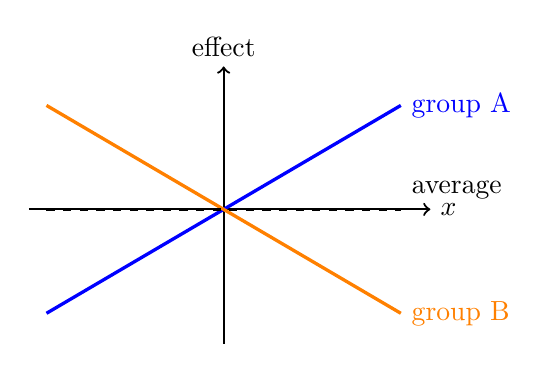
\begin{tikzpicture}[x=0.75cm,y=0.55cm]
\draw[->,thick] (-3.3,0) -- (3.5,0) node[right] {$x$};
\draw[->,thick] (0,-3.1) -- (0,3.3) node[above] {effect};
\draw[blue,very thick] (-3,-2.4) -- (3,2.4) node[right] {group A};
\draw[orange,very thick] (-3,2.4) -- (3,-2.4) node[right] {group B};
\draw[black,dashed,very thick] (-3,0) -- (3,0) node[above right] {average};
\end{tikzpicture}
\spacer[0.25]
\textbf{Flat average $\neq$ no model effect}
}
\end{framev}


\begin{framev}[align=top]{RHALE: Robust and Heterogeneity-aware ALE}
RHALE builds on DALE's local gradients and extends the idea in two directions.
\spacer[0.25]
\splitVTT[0.5]{
\spacer[0.6]
\begin{itemizeM}
\item \textbf{Heterogeneity-aware}
\begin{itemizeS}
\item Shows the average local effect
\item Also summarizes how much instance-level effects vary around that average
\item Helps distinguish a genuinely small effect from cancellation of opposing effects
\end{itemizeS}
\end{itemizeM}
}{
\spacer[0.6]
\begin{itemizeM}
\item \textbf{Robust adaptive binning}
\begin{itemizeS}
\item Uses wider bins where local effects are nearly constant
\item Uses narrower bins where the effect changes and sufficient data are available
\item Balances approximation bias against sampling variance
\end{itemizeS}
\end{itemizeM}
}
\spacer[0.25]
\textbf{Why adaptive bins matter:}
\[
\underbrace{\sigma_*^2}_{\text{observed within-bin spread}}
=
\underbrace{\sigma^2}_{\text{effect heterogeneity}}
+
\underbrace{\mathcal{E}^2}_{\text{within-bin approximation error}}.
\]
Fixed bins can therefore overstate heterogeneity. RHALE reports local-effect spread itself---not spread divided by $\sqrt{n_k}$ and not a confidence interval.
\end{framev}


\begin{framev}[fs=small,align=top]{ALE, DALE, and RHALE at a Glance}
\begin{center}
\renewcommand{\arraystretch}{1.4}
\begin{tabular}{p{0.235\textwidth} p{0.195\textwidth} p{0.195\textwidth} p{0.215\textwidth}}
\toprule
\textbf{Question} & \textbf{ALE} & \textbf{DALE} & \textbf{RHALE} \\
\midrule
Estimator of local signal & Finite differences & Gradients & Gradients \\
Model requirement & Any prediction model & Gradients required for benefit & Gradients preferred \\
Artificial points & At bin boundaries & No with gradients & No with gradients \\
Bin choice & Fixed by user & Fixed by user & Adaptive \\
Shows heterogeneity & Optional, but bin-sensitive & SE of mean effect & Explicit, adaptive \\
Main strength & General and dependency-aware & Fast, reusable, on-data & Average effect plus hidden variation \\
\bottomrule
\end{tabular}
\end{center}
\spacer[0.25]
\textbf{Rule of thumb:} Use ALE for model-agnostic black boxes. With gradients, DALE efficiently estimates the mean effect; RHALE builds on DALE when adaptive bins and heterogeneity are also needed.
\end{framev}


\begin{framev}[align=top]{Limitations and Responsible Interpretation}
\begin{itemizeM}
\item \textbf{Descriptive by default:} The methods explain a fitted model over an observational distribution. A causal interpretation requires a separate identification argument; conditional averaging is not itself an intervention.
\item \textbf{Data-distribution dependent:} Effects describe the fitted model over the observed feature distribution and may change under dataset shift.
\item \textbf{Finite support:} Sparse regions remain difficult; inspect bin counts and stability across reasonable settings.
\item \textbf{Effect decomposition can be unintuitive:} With dependent, interacting features, a first-order ALE curve can absorb part of an interaction and need not match the formula's main-effect shape. \furtherreading{GROEMPING2020}
\item \textbf{Global summaries:} ALE and DALE can hide interactions; RHALE signals heterogeneity but does not automatically identify its source or the relevant subgroups.
\item \textbf{RHALE choices remain:} Its automatic binning has hyperparameters, and very small datasets may require adjustment.
\end{itemizeM}
\spacer[0.25]
\textbf{Good practice:} Interpret effect shape, data support, uncertainty, and heterogeneity together.
\end{framev}


\begin{framev}[align=top]{Conclusions and Further Reading}
\begin{itemizeM}
\item \textbf{ALE:} Strong baseline for feature effects with dependent features. \furtherreading{APLEYZHU2020}
\item \textbf{DALE:} Replaces boundary perturbations with gradients at observed points, while retaining a within-bin approximation. \furtherreading{GKOLEMIS2023DALE}
\item \textbf{RHALE:} Builds on DALE and adds heterogeneity information plus adaptive binning. \furtherreading{GKOLEMIS2023RHALE}
\item \textbf{Regional follow-up:} REPID and RegionalRHALE search for subgroups with more homogeneous effects. \furtherreading{HERBINGER2022} \furtherreading{EFFECTOR2024}
\item \textbf{Software:} The \texttt{effector} Python package implements ALE and RHALE. \furtherreading{EFFECTOR}
\end{itemizeM}
\spacer[0.25]
\textbf{Take-away:} Before trusting a smooth global curve, ask whether its approximation is stable and whether averaging hides important local differences.
\end{framev}

\endlecture
\end{document}
